\documentclass{article}
\usepackage{graphicx} % Required for inserting images
\usepackage{comment}
\usepackage{amsmath}
\usepackage{amssymb}
\usepackage{hyperref}
\usepackage{url}
\usepackage[
    backend=biber,
    style=authoryear,   % Name-Year style
    sorting=nyt,
    natbib=true         % <--- Add this to enable \citep and \citet
]{biblatex}
\addbibresource{biblio.bib}
%\usepackage{draftwatermark}
%\SetWatermarkText{DRAFT}
%\SetWatermarkScale{2.5}

\graphicspath{{./}{figures/}{SI_figures/}{img/}}

\title{Convective Organization as Markov Trajectories in Latent Space}
\author{Sophie Abramian, Olivier Pauluis, Pierre Gentine}
\date{December 2025}

\begin{document}

\maketitle


\section*{Abstract}
High-dimensional dynamical systems, such as convective storms, pose fundamental challenges for reduced-order modeling due to their complex, stochastic evolution across multiple scales. We present a data-driven framework for stochastic reduced-order modeling of convective dynamics that combines Koopman operator theory with discrete-state Markov chains. The method learns low-dimensional representations of convective mass flux directly from high-resolution simulations by encoding isentropic mass-flux profiles into a latent space where evolution is approximated as linear and probabilistic. Applied to cloud-resolving simulations under fixed vertical wind shear, the framework identifies an eight-dimensional latent manifold that captures convective variability through transitions between a small number of dominant states. The learned Markov transition matrices reveal regime-dependent pathways and clear distinctions between weakly and strongly organized convection. Deviations from Markovianity in organized regimes expose the role of internal feedbacks—particularly cold-pool dynamics—as sources of effective memory. Conditioning the state space on cold-pool intensity restores Markovian behavior, demonstrating that explicitly embedding internal processes improves model fidelity. The results indicate that convective diversity arises from the range of dynamical trajectories supported by the environment rather than from distinct states alone.

\section{Introduction}

High-dimensional dynamical systems — defined by many nonlinearly coupled degrees of freedom whose interactions produce complex, often stochastic evolution — arise across the physical sciences. Convective storms are a canonical example: their dynamics involve multiscale couplings between thermodynamics, fluid motion, and microphysics, encoded in high-dimensional state variables from satellite observations \citep{hu2020observed, fiolleau2024database} or cloud-resolving simulations \citep{feng2025mesoscale}. Despite this complexity, convection exerts outsized control on vertical mass, energy, and moisture transport, making its representation in coarse-grained climate models a persistent challenge, especially under warming \citep{yang2023impact, bolot2025no, prein2022towards, chakraborty2023overview}.

The high dimensionality of convective systems has historically motivated drastic simplifications. Stochastic multi-cloud models \citep{khouider2006multicloud, majda2008stochastic, khouider2010stochastic} demonstrated that convective populations can be approximated as a Markov chain over a small number of prescribed cloud types — shallow, congestus, and deep — with transition rules on a coarse lattice. This framework captures the birth, growth, and decay of storm populations and horizontal variability in cloud cover. However, precisely because the states are chosen a priori rather than learned from the data, these models cannot represent the diversity of vertical mass-flux profiles that arise for a given cloud geometry. The limitation matters most during extreme events \citep{MullerYukari19}, where the dynamical component controls precipitation change \citep{singh2012upward, abramian2023extreme, wang2022convective}: bottom- or top-heavy vertical structures strongly influence the duration and intensity of extreme rainfall \citep{li2025bimodal}.

More generally, low-dimensional descriptions of high-dimensional systems are often weakly connected to the underlying dynamics: the variables chosen to describe the flow are not necessarily the variables in which the dynamics simplify. Koopman operator theory \citep{koopman1931hamiltonian, brunton2021modern} offers a principled resolution to this problem. Rather than seeking a reduced model directly in the space of physical variables — where nonlinear couplings make any low-dimensional truncation dynamically inconsistent — one constructs observables, nonlinear transformations of the physical state, in which the dynamics become exactly linear. The nonlinear complexity is not eliminated but transferred to the geometry of the observable space, so that the projected evolution is linear by construction, regardless of the complexity of the original system. In practice, these observables must be approximated from data. Recent work recasts this as a representation-learning problem \citep{lusch2018deep}: an encoder maps the physical state into a latent space where dynamics are constrained to be linear, while a decoder ensures fidelity to the original state. The approach extends to chaotic and stochastic dynamics \citep{nathaniel2026generative}.

We adopt this framework and make two specific choices that define our approach. First, we represent the convective flow in isentropic coordinates \citep{pauluis2013isentropic}. Isentropic analysis reorganizes mass flux according to equivalent potential temperature, yielding a thermodynamically consistent description that preserves energetic structure and filters reversible adiabatic motions. This provides a high-dimensional, physically grounded input to the encoder — not itself a reduced representation, but a structured substrate from which dynamically relevant observables can be extracted.

Second, we depart from Koopman autoencoders that enforce deterministic linear dynamics. Instead, we partition the learned latent space into a finite set of discrete states through clustering \citep{kaiser2014cluster, souza2024representing}, and model transitions between them probabilistically. The resulting reduced-order model is a Markov chain on state occupation probabilities: finite-dimensional, linear, and memoryless by construction. Unlike existing stochastic convection models, the discrete states are neither prescribed nor heuristic — they are learned jointly with the encoding.

This construction bridges two traditions. Stochastic multi-cloud models operate on prescribed states with limited dynamical diversity. Koopman autoencoders learn expressive representations but typically enforce deterministic dynamics. By combining learned discrete states with stochastic transitions, we obtain a model that is both physically interpretable and consistent with the irreducibly stochastic character of convective evolution.

We apply this framework to squall lines simulated with the System for Atmospheric Modeling (SAM) under controlled large-scale forcing, and address three questions: (i) What are the dominant convective mass-flux states accessible under a given forcing, here characterized by vertical wind shear? (ii) Can transitions between these states be modeled as a Markov chain, and do transition pathways differ between weakly and strongly organized convection? (iii) To what extent is convective variability memoryless, and where do internal feedbacks — cold-pool dynamics in particular — introduce effective memory?

Section 2 describes the methodology. Section 3 presents results. Section 4 discusses implications for convective modeling and concludes.

\section{Methods}

\subsection{Idealized cloud-resolving simulations}

To examine the response of convection to fixed vertical wind shear, we perform idealized cloud-resolving simulations using the System for Atmospheric Modeling (SAM) \cite{khairoutdinov2003}. Following \cite{muller2013impact}, a low-level shear profile is imposed following previous idealized studies (see also \cite{rotunno1988theory, houze1977structure, robe2001effect}). The wind profile is linear, with a basal velocity of $8.5\,\mathrm{m\,s^{-1}}$ and a shear depth of $1\,\mathrm{km}$. This value is deliberately suboptimal relative to the shear magnitude ($\sim10\,\mathrm{m\,s^{-1}}$) that maximizes convective organization, in order to enhance sensitivity to internal variability (\cite{abramian2022shear}). In this regime, the balance between shear and cold-pool dynamics is more unstable, and variations in cold-pool properties exert a substantial control on convective development.

The model domain spans $128\,\mathrm{km} \times 128\,\mathrm{km}$ horizontally and extends from the surface to $17\,\mathrm{km}$ in the vertical, with enhanced resolution in the boundary layer. A sponge layer is applied near the model top to absorb upward-propagating gravity waves. Microphysical processes are represented using a single-moment scheme. The simulation is first integrated for 30 days to reach radiative--convective equilibrium and then continued for an additional 27 days for analysis. Model output is saved at 2-min intervals, yielding approximately $2\times10^{4}$ time steps, and includes both two- and three-dimensional fields. Under the imposed shear, convection self-organizes into squall-line structures oriented perpendicular to the shear direction, as illustrated in Fig.~\ref{fig:simu_isentrop}. The system alternates between quiescent phases and episodes of strong organization. Despite identical large-scale forcing, pronounced variability emerges in the structure, intensity, and persistence of the organized convective systems.

\subsection{Isentropic mass flux analysis and preprocessing}

Vertical transport associated with moist convection is inherently three-dimensional, intermittent, and multiscale. When diagnosed directly in physical space, the vertical mass flux reflects the superposition of contributions from convective updrafts and downdrafts, gravity waves, compensating subsidence, and turbulent fluctuations. This combination produces a noisy, high-dimensional field, making it difficult to isolate the collective transport by convection or to compare it consistently across realizations.

A physically grounded reduction of this complexity is provided by isentropic analysis \cite{pauluis2013isentropic}. Rather than organizing vertical motion by spatial location, this approach conditions transport on thermodynamic variables that are approximately conserved following moist adiabatic motion \cite{chen2022crucial}. In the moist atmosphere, we approximate isentropic surfaces using the moist static energy variable $h$. Projecting the vertical mass flux onto $h$ therefore reorganizes transport according to the energetic content of moving air parcels, rather than their instantaneous spatial position.

We define the moist static energy and the associated vertical isentropic mass flux as
\begin{align}
    h(x,y,z,t) & = c_p\, T(x,y,z,t)+ g\, z + L_v\, q_v(x,y,z,t),\\ 
    M(h,z,t) &= \int_{0}^{N_x}\int_{0}^{N_y} \rho(z,t)\,w(x,y,z,t)\,
    \delta\!\left(\hat{h}(x,y,z,t)-h\right)\,dx\,dy,
\end{align}
where $h(x,y,z,t)$ denotes the moist static energy, $c_p$ is the specific heat capacity of air at constant pressure, $T(x,y,z,t)$ is the absolute temperature, $g$ is the gravitational acceleration, $z$ is height, $L_v$ is the latent heat of vaporization, and $q_v(x,y,z,t)$ is the water vapor mixing ratio. The quantity $M(h,z,t)$ denotes the vertical isentropic mass flux, defined as the horizontal integral of the vertical mass flux $\rho(z,t)\,w(x,y,z,t)$ projected onto moist static energy levels using the Dirac delta function $\delta(\cdot)$. Here $\rho(z,t)$ is the air density, $w(x,y,z,t)$ is the vertical velocity, $\hat{h}(x,y,z,t)$ denotes the local moist static energy field, and $N_x$ and $N_y$ are the horizontal domain dimensions.

This thermodynamic conditioning performs two key functions. First, it reduces dimensionality by collapsing horizontal spatial variability into a compact $(h,z)$ phase space that retains the dominant structure of vertical transport. Second, it separates dynamically distinct processes that overlap in physical space but differ in thermodynamic character. Convective updrafts preferentially transport high $h$ air upward, entraining and evaporatively cooled downdrafts populate lower $h$ levels, while gravity-wave motions—characterized by weak net thermodynamic transport—are confined to low $h$ regions of the phase space\citep{chen2018atmospheric, chen2020significant}.

Within this isentropic representation, vertical transport organizes into coherent and interpretable patterns \citep{mrowiec2016isentropic}. Sustained positive mass flux at high $h$ extending through the troposphere is characteristic of deep convection, while shallow convection appears as weaker transport rapidly diluted by entrainment. Precipitating systems exhibit enhanced downdraft signatures and broadened $h$ distributions, and cold-pool dynamics manifest as near-surface, low-$h$ mass flux associated with evaporative cooling.

\begin{figure}
    \centering
    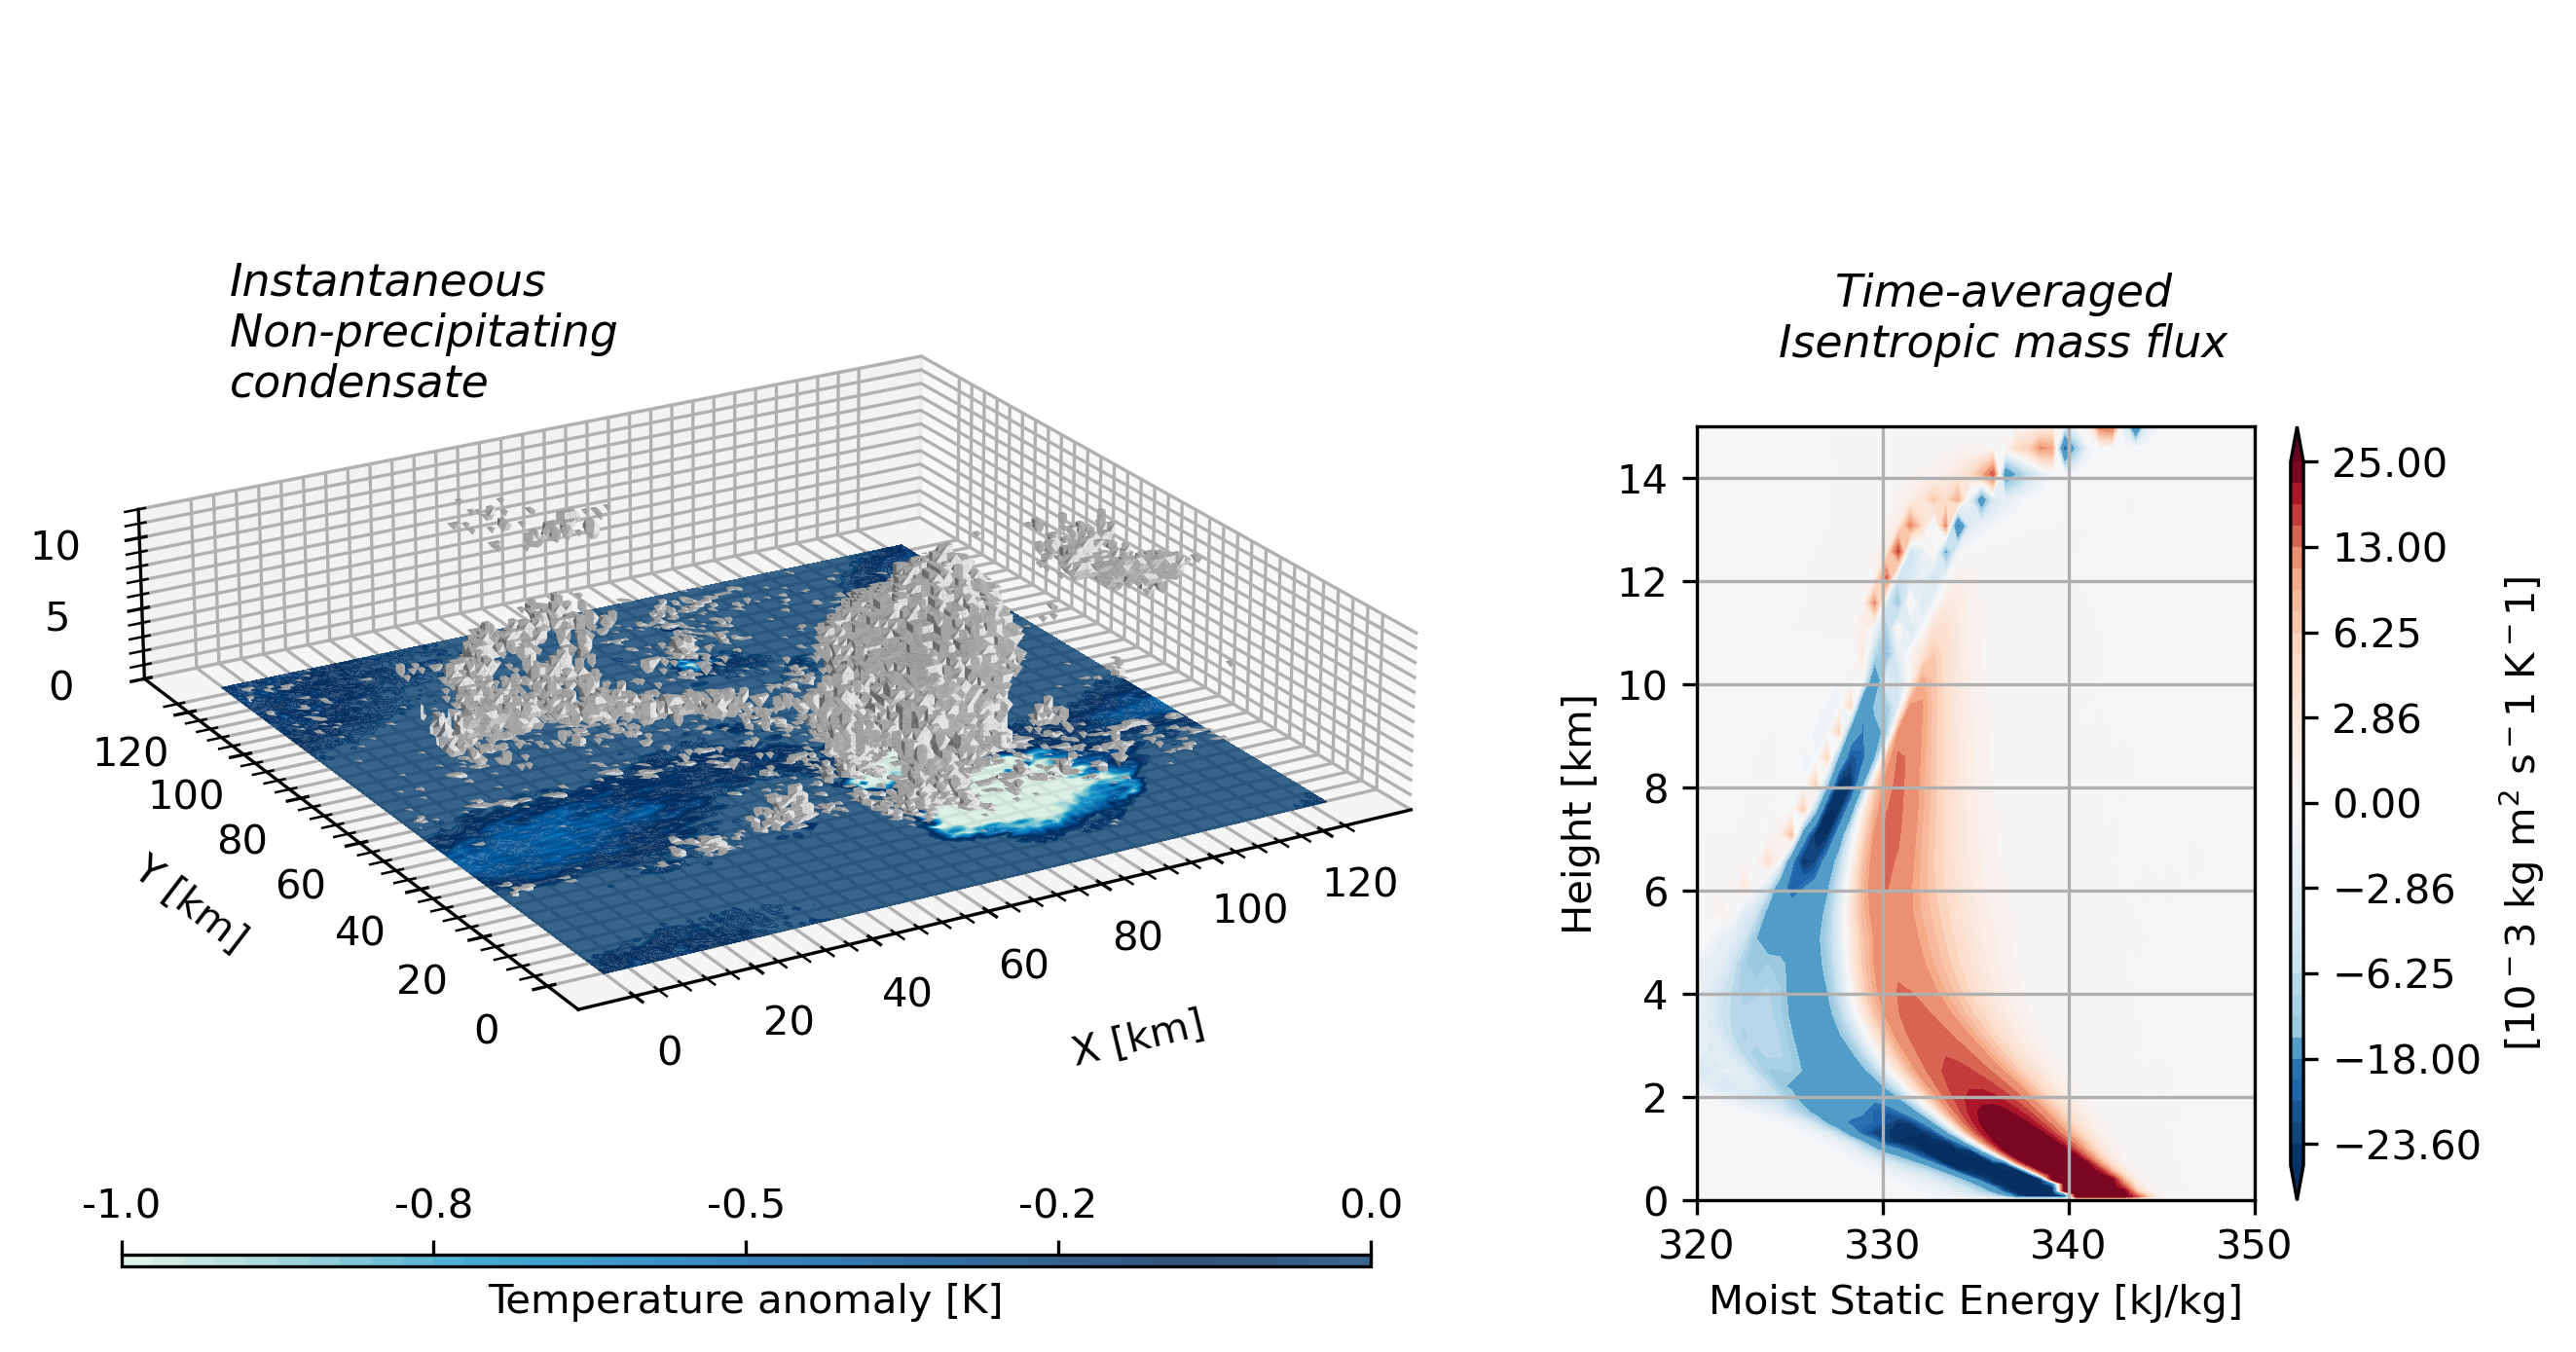
\includegraphics[width=\linewidth]{img_004015.png}
    \caption{A. Snapshot of the isovolume of non precipitating condensate (QN) at the levels 0f 0.02 kg/kg in volume and the surface temperature anomaly, the white zone corresponding to a cold pool. B. Time average over 27 days with 2min resolution of the isentropic mass flux.}
    \label{fig:simu_isentrop}
\end{figure}

The learning dataset is constructed from the time series of isentropic mass flux fields spanning 27 days with 2-minute temporal resolution. Moist static energy $h$ is discretized into 48 bins ranging from 320 to 350~kJ~kg$^{-1}$, and the vertical coordinate corresponds to the first 48 model levels, spanning altitudes from approximately 25~m to 16~km. The resulting raw dataset has dimensions $(n_t \approx 2\times10^{4},\, n_h=48,\, n_z=48)$. For each spatial pixel, the temporal mean is removed to suppress the stationary background signal and isolate transient variability. A spatial mask is then applied to retain only pixels that exhibit nonzero values at least once over the full time series, thereby discarding invariant regions of the domain; this is particularly important at higher altitudes, where the admissible range of $h$ progressively shrinks. The retained fields are subsequently reshaped into vectors. To enhance weak signals while preserving amplitude ordering, a signed logarithmic transform,
\[
\mathrm{sign}(x)\,\log(1+|x|),
\]
is applied to the masked values. The resulting mean-centered, masked, log-transformed vectors constitute the input representation used to train the model.

Given the time-ordered sequence of processed state vectors $\{X_t\}$, each training sample consists of a pair $(X_t, X_{t+\Delta t})$ separated by a fixed temporal offset $\Delta t = 5$. The full dataset is randomly permuted and split into a training set (90\%) and a validation set (9.9\%), with the remaining fraction excluded from optimization. During training, samples are drawn in mini-batches of size 256 and randomly shuffled at each epoch to decorrelate temporal ordering within batches, whereas the validation set is iterated deterministically.

\subsection{Reduced-order stochastic model}

The function of the designed model is not only to reduce the dimensionality of isentropic mass-flux diagrams, but to construct a dynamical, probabilistic representation of convective evolution. Specifically, we seek a reduced representation that (i) encodes the essential physical structure of convection, (ii) enables a meaningful partitioning of convective configurations into discrete states, and (iii) allows us to predict how convection is likely to evolve in time within this reduced space.

To this end, we introduce a reduced-order stochastic model that combines a variational autoencoder (VAE), a data-driven latent-state representation, and a discrete-time Markov transition model (Fig.~\ref{fig:model}). Rather than treating dimensionality reduction and temporal modeling as separate steps, the model is trained jointly so that the learned latent representation is both physically meaningful and dynamically predictive.

\begin{figure}
    \centering
    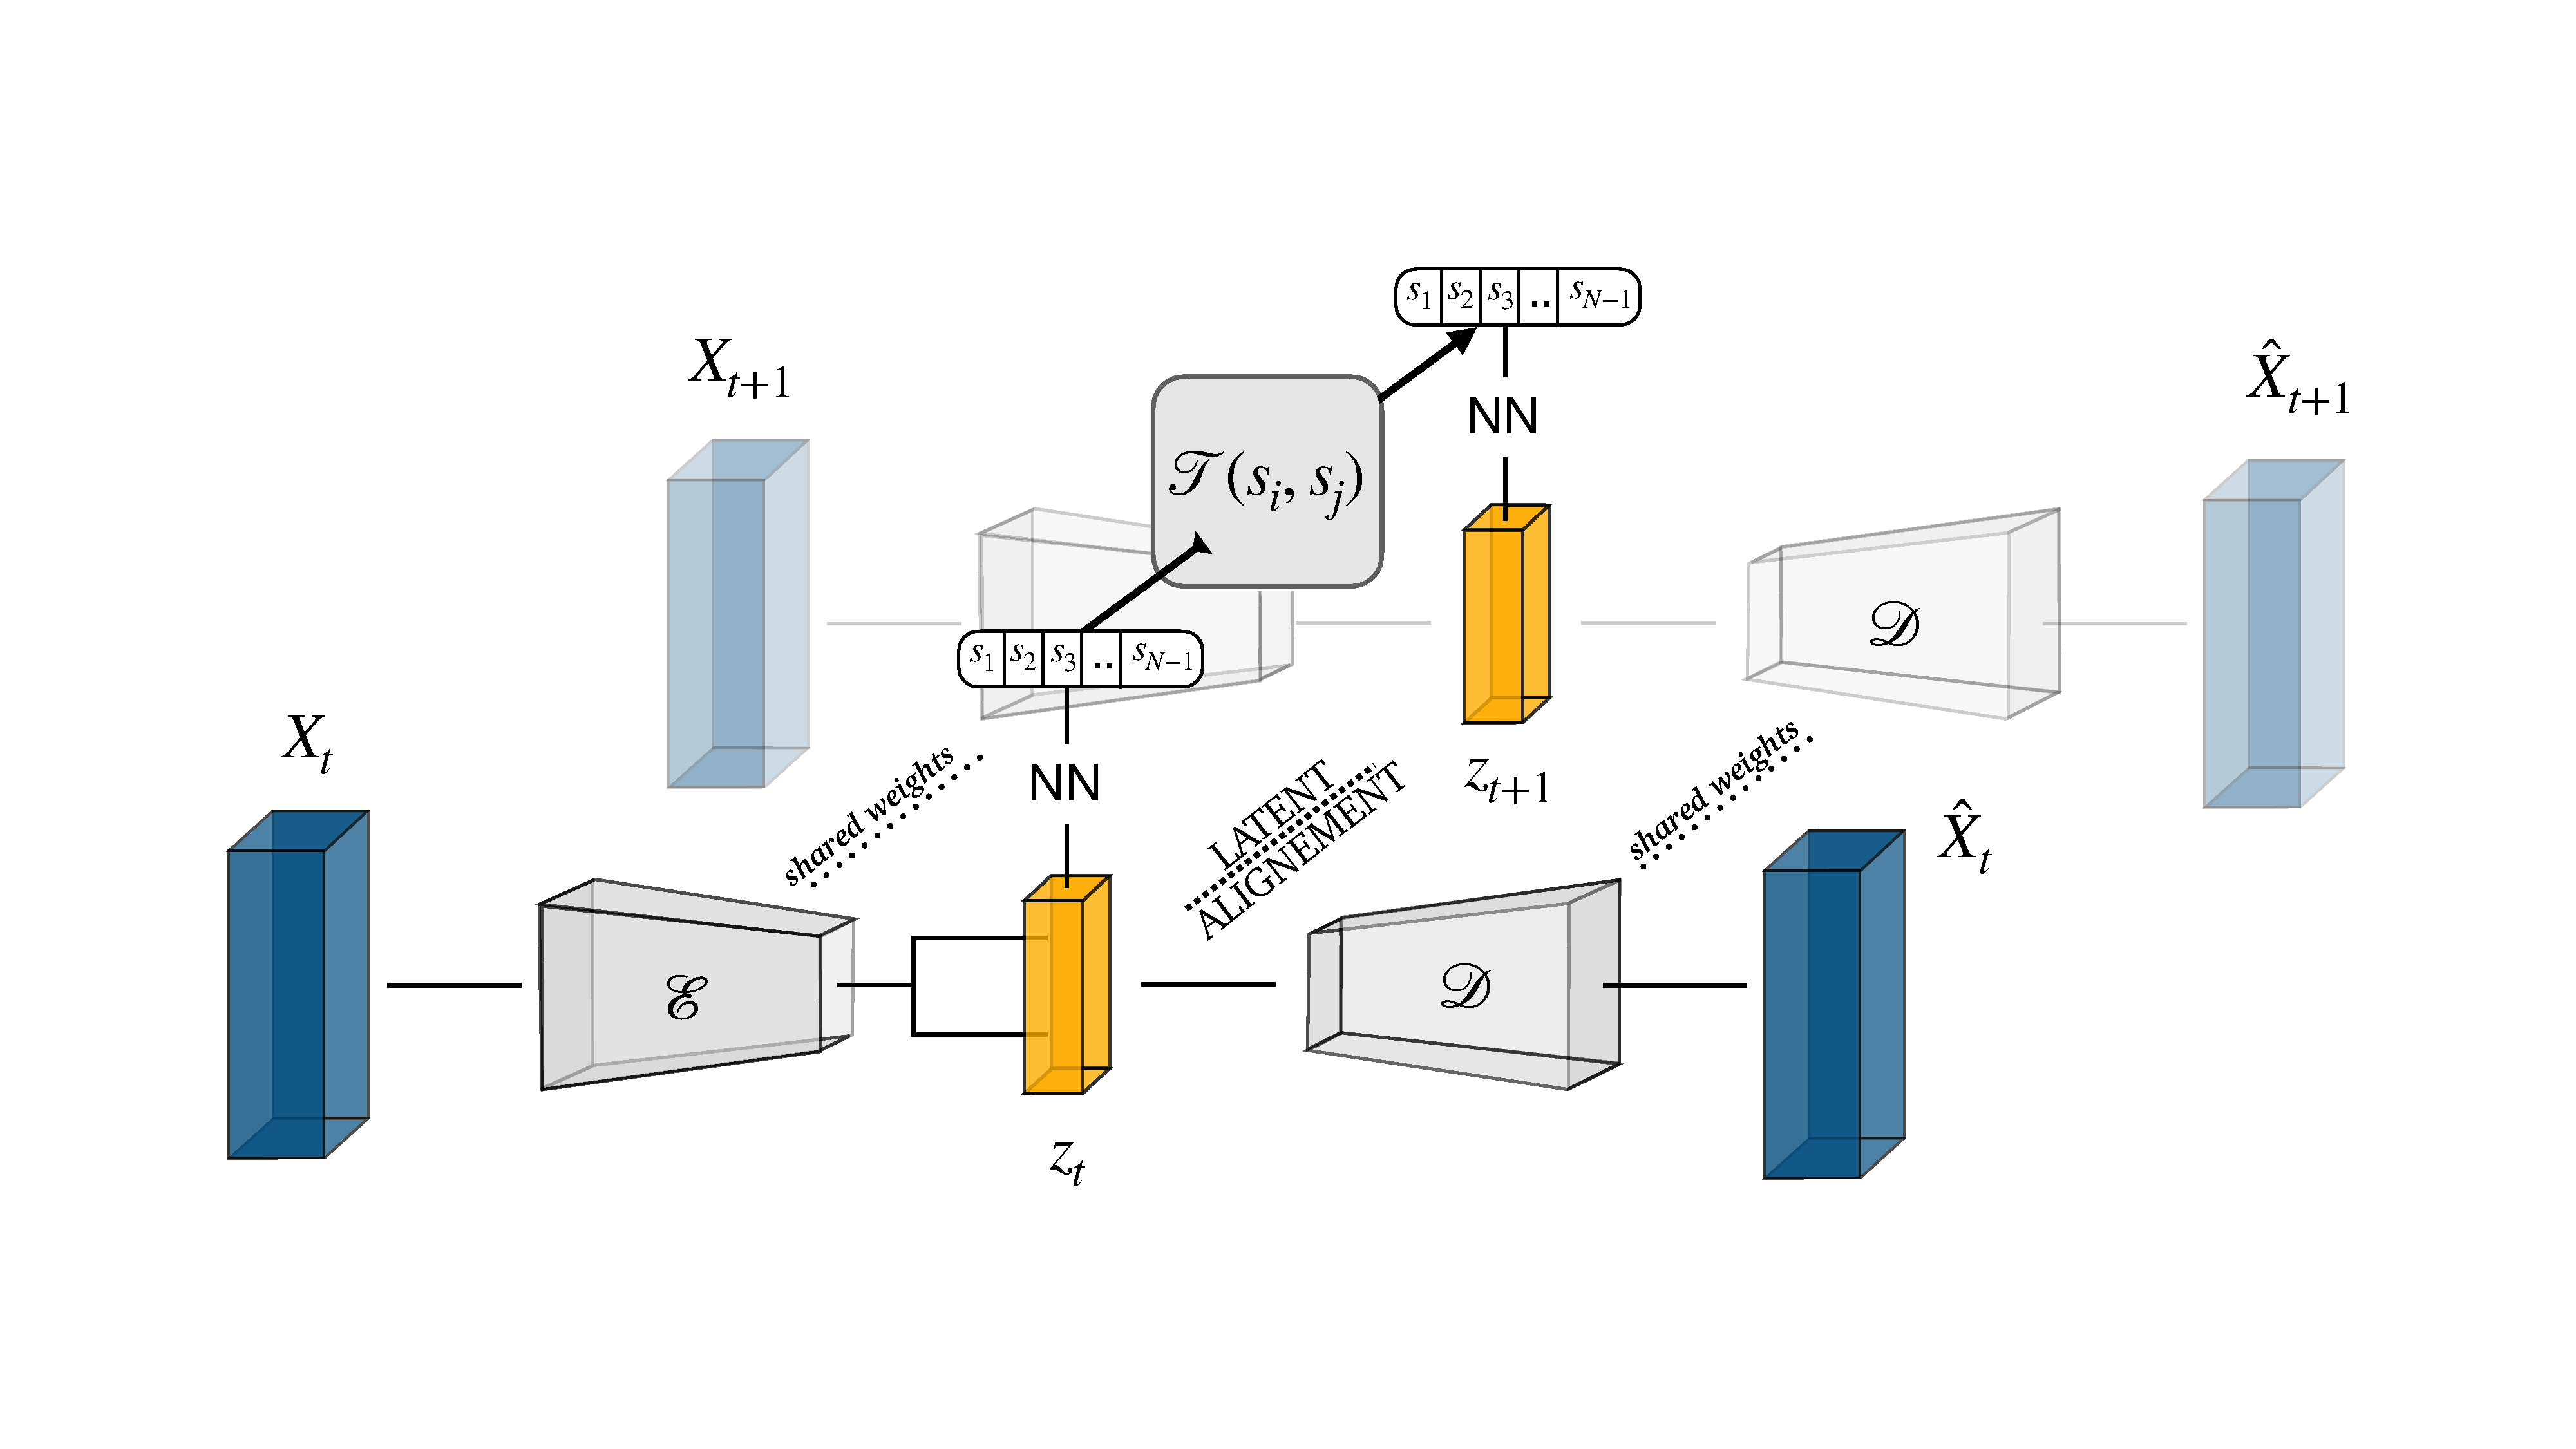
\includegraphics[width=0.9\linewidth]{model_vae_mc.pdf}
    \caption{\textbf{Model description.} The model combines a variational autoencoder (VAE) with a Markovian state assignment and transition framework. An encoder maps the input data to a latent representation $z_t$, which is reconstructed by a decoder. A neural network assigns to each latent vector $z_t$ a probability distribution over a finite set of discrete states. Temporal evolution in latent space is modeled by a linear transition operator $T$, which predicts the state distribution at time $t+1$ from the state distribution at time $t$. During training, consecutive latent vectors $(z_t, z_{t+1})$ are jointly considered: the VAE is trained using a reconstruction loss, while the transition operator is trained by comparing the predicted state distribution $T\,s(z_t)$ with the state distribution inferred from $z_{t+1}$.}
    \label{fig:model}
\end{figure}

\subsubsection{Variational autoencoder Backbone}

Each isentropic mass-flux diagram at time $t$, denoted $X_t$, is encoded into a low-dimensional latent representation using a variational autoencoder. The encoder maps $X_t$ to a Gaussian distribution in latent space,
\[
q(z \mid X_t) = \mathcal{N}(\mu, \sigma^2),
\]
where $\mu$ and $\sigma$ denote the mean and standard deviation of the $d$-dimensional latent variables. A latent sample $z$ drawn from this distribution is then decoded to produce a reconstruction $\hat{X}_t$ of the original diagram. Regularization of the latent variables is enforced through a Kullback--Leibler divergence penalty that constrains the learned posterior toward a unit Gaussian prior. This variational constraint yields a smooth latent space in which nearby points correspond to similar convective configurations, enabling meaningful interpolation and supporting a stable, probabilistic description of convective evolution.

\subsubsection{Latent Space Partitioning}

The continuous latent representation is mapped onto a finite set of $K=7$ discrete convective states through a neural network that performs a soft partitioning of latent space. The number of clusters is found empirically and a sensitivity test can be found in Supplementary Information. At each time $t$, the model outputs a probability vector
\[
s_t = \{ s_t(1), \ldots, s_t(K) \},
\]
where $s_t(k)$ denotes the probability that the system occupies state $k$. This mapping can be interpreted as a data-driven clustering mechanism, in which close latent representations are grouped into dynamically meaningful regimes, although this clustering actually affect and shape the latent space in return. The assignment is probabilistic rather than deterministic, allowing for uncertainty and overlap between states, which is essential in transitional or weakly organized configurations.

To prevent state collapse—whereby most samples are assigned to a small subset of states—we regularize the state assignment using a contrastive objective that encodes prior physical knowledge about the input. Specifically, we introduce a contrastive loss based on the structural similarity of isentropic mass-flux anomaly fields. Each sample is discretized into three regions using fixed thresholds $\{-1.5,\,1.5\}$, corresponding to negative anomalies, near-neutral values, and positive anomalies. From these regions, binary masks are constructed and compared using a macro-averaged Dice coefficient, which measures the spatial overlap of positive and negative anomaly structures while intentionally discarding information about anomaly amplitude or fine-scale intensity. For randomly sampled pairs $(i,j)$ within a batch, the Dice similarity $\mathrm{Dice}(i,j)$ defines a notion of physical proximity. Pairs with high structural similarity are encouraged to share the same latent state, while structurally dissimilar pairs are encouraged to occupy different states. This is implemented through a soft contrastive loss that penalizes disagreement for similar pairs (cohesion) and agreement for dissimilar pairs (separation), with a smooth transition between the two regimes. An additional mid-range penalty discourages uncertain assignments when the similarity is ambiguous. We denote this loss term as $\mathcal{L}_{\mathrm{Dice}}$ (details in Supplementary Information).

\subsubsection{Markov transition dynamics}

We assume that, at the temporal resolution of the simulations, the evolution of convection can be approximated as a first-order Markov process in state space. The transition probabilities are encoded in a transition matrix $T$, defined by
\[
T_{ij} = P(s_{t+\Delta t} = j \mid s_t = i).
\]
This matrix captures the persistence of convective regimes, preferred transitions between states, and rare events such as the spontaneous onset or decay of organized convection. The model is designed to receive consecutive timesteps as input, $X_t$ and $X_{t+\Delta t}$, which are encoded using the same encoder into $z_t$ and $z_{t+1}$. The neural network that assigns states based on the latent space returns $s_t$ and $s_{t+\Delta t}$. The transition matrix is trained to predict $\hat{s}_{t+\Delta t} = T\cdot s_t$ in comparison to $s_{t+\Delta t}$.

\subsubsection{Joint optimization}

The VAE, neural state-assignment network, and Markov transition matrix are trained jointly by minimizing the composite loss function
\[
\mathcal{L} =
\|X - \hat{X}\|^2
+
\frac{1}{2}\sum_{i=1}^d
\left(
\mu_i^2 + \sigma_i^2 - \log \sigma_i^2 - 1
\right)
-
\mathcal{L}_{\mathrm{Dice}}
-
\sum_{i,j}
s_t(i)\, s_{t+1}(j)\, \log T_{ij}.
\]

The first term is the reconstruction loss, ensuring that the reduced representation preserves the dominant spatial structure of the isentropic mass-flux diagrams. The second term is the Kullback--Leibler divergence between the learned latent distribution and a unit Gaussian prior, which regularizes the latent space and enforces continuity. The third term is the Dice-based contrastive loss that promotes physically coherent and balanced state assignments while preventing collapse onto a small number of regimes. The final term is the negative log-likelihood of observed state transitions under the Markov model and enforces dynamical consistency between consecutive time steps.

Together, these loss components ensure that the learned convective states are physically interpretable, statistically regularized, and dynamically predictive. The resulting framework provides a compact stochastic representation of convective variability, in which organized convection emerges as a probabilistic outcome constrained—but not uniquely determined—by the large-scale environment.

Optimization is performed with AdamW (learning rate $5 \times 10^{-5}$, batch size $256$) for $512$ epochs, with gradient norm clipping at $1.0$. All loss components are accumulated as batch-size--weighted averages at the epoch level, and the best model is selected based on the minimum validation total loss. Detailed training, validation, and test loss decompositions, reconstruction diagnostics, and latent-space statistics are provided in the Supplementary Information.



\section{Results}

\subsection{Physical interpretation of the latent space}

The model compresses time series of isentropic mass-flux fields—used here as a compact description of the convective state—into a time series of latent vectors $\mathbf{z}(t)\in\mathbb{R}^8$. Each time step is subsequently assigned to a discrete convective state.

\paragraph{Latent-space structure revealed by PCA.}

The variational autoencoder is trained to reconstruct the mass-flux fields while regularizing the latent distribution toward an isotropic Gaussian prior. As a result, individual latent coordinates have no intrinsic physical meaning, and physically relevant variability is not expected to align with single latent dimensions.

To extract the dominant modes of variability in the learned representation, we apply principal component analysis (PCA) to the latent vectors $\mathbf{z}(t)$. The resulting projection reveals a structured organization in which discrete convective states occupy distinct regions of the dominant variance subspace (Fig.~\ref{fig:clusters}). The first two principal components explain $22\%$ and $17\%$ of the total latent variance, respectively, indicating that a limited number of emergent degrees of freedom captures a substantial fraction of the learned variability. A three-dimensional PCA projection, shown in the Supplementary Material, confirms that clusters with apparent overlap in two dimensions are separated along higher-order components.

\begin{figure}
    \centering
    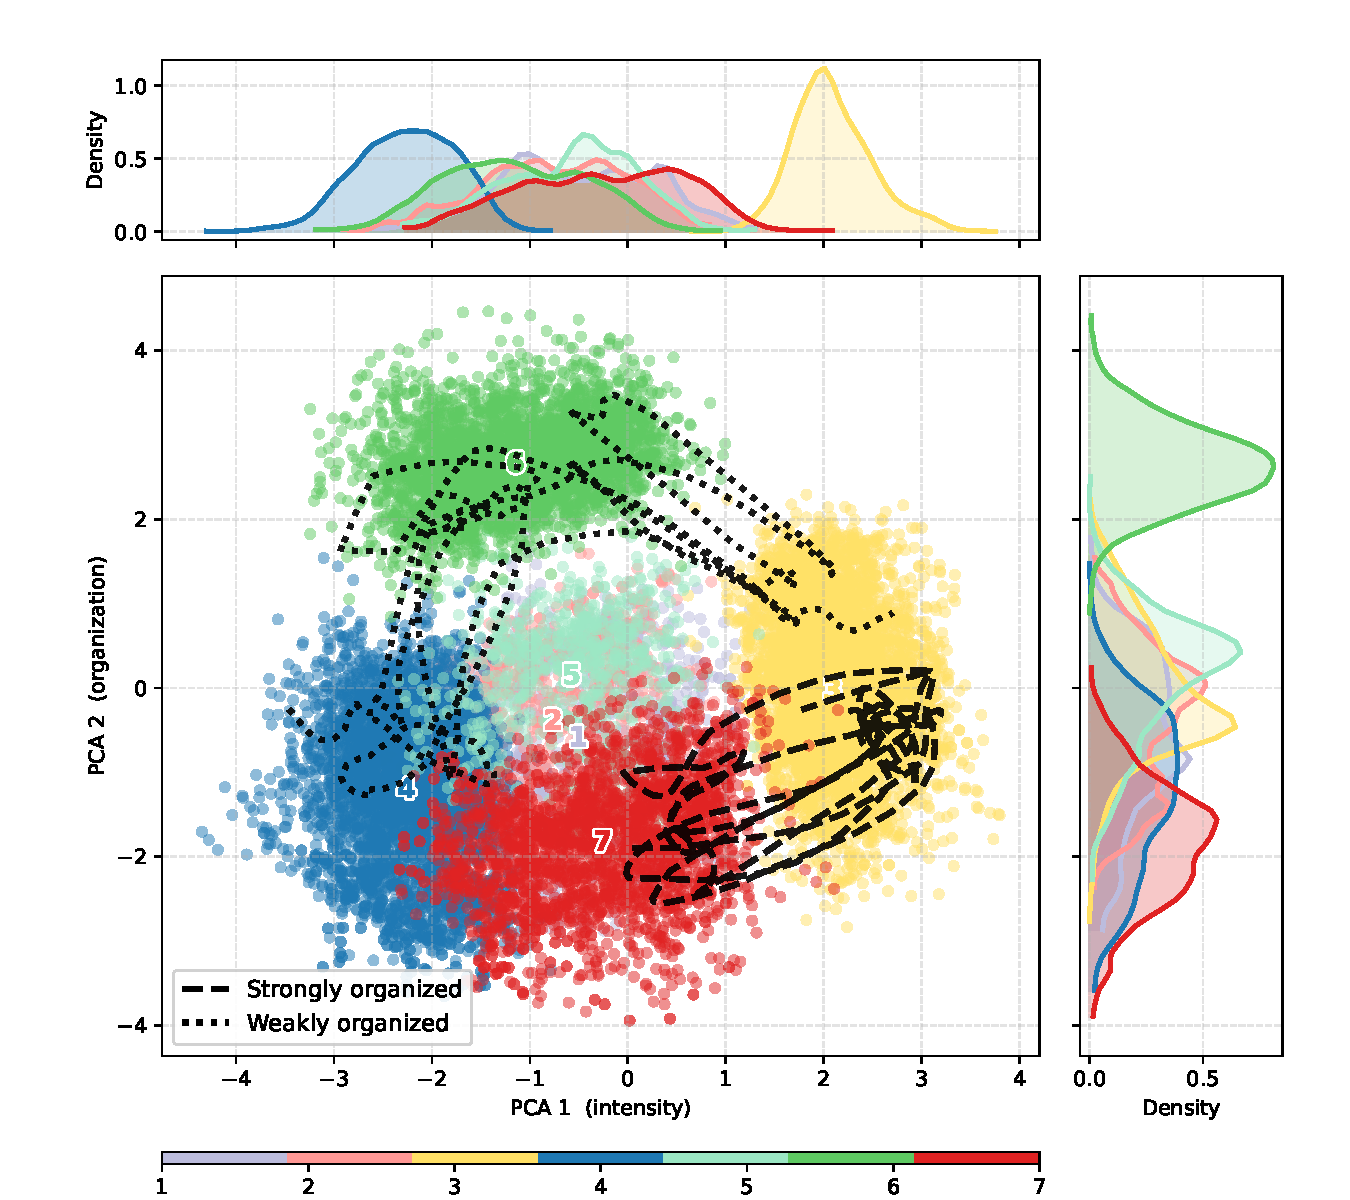
\includegraphics[width=0.75\textwidth]{clusters.pdf}
    \caption{\textbf{Latent-space organization.} PCA projection of the latent space colored by cluster assignment. Each point corresponds to one time step; trajectories illustrate the time evolution over 5~h.}
    \label{fig:clusters}
\end{figure}

\paragraph{Emergent axes: convective life cycle and organization.}

The physical interpretation of the dominant latent directions is obtained by relating the principal components to independent diagnostics of convection (Fig.~\ref{fig:axis_var}). The first principal component is strongly correlated with domain-mean precipitation, indicating that it primarily captures convective intensity and progression along the convective life cycle, from weak or suppressed states to vigorous, precipitating convection.

In contrast, the second principal component shows little correlation with precipitation but is strongly anticorrelated with a measure of cloud spatial organization derived from the variance of precipitable water. Variability along this axis therefore reflects differences in convective organization rather than intensity. The near-orthogonality of the two components indicates that convective intensity and spatial organization emerge as largely independent modes of variability in the learned representation.

\begin{figure}
    \centering
    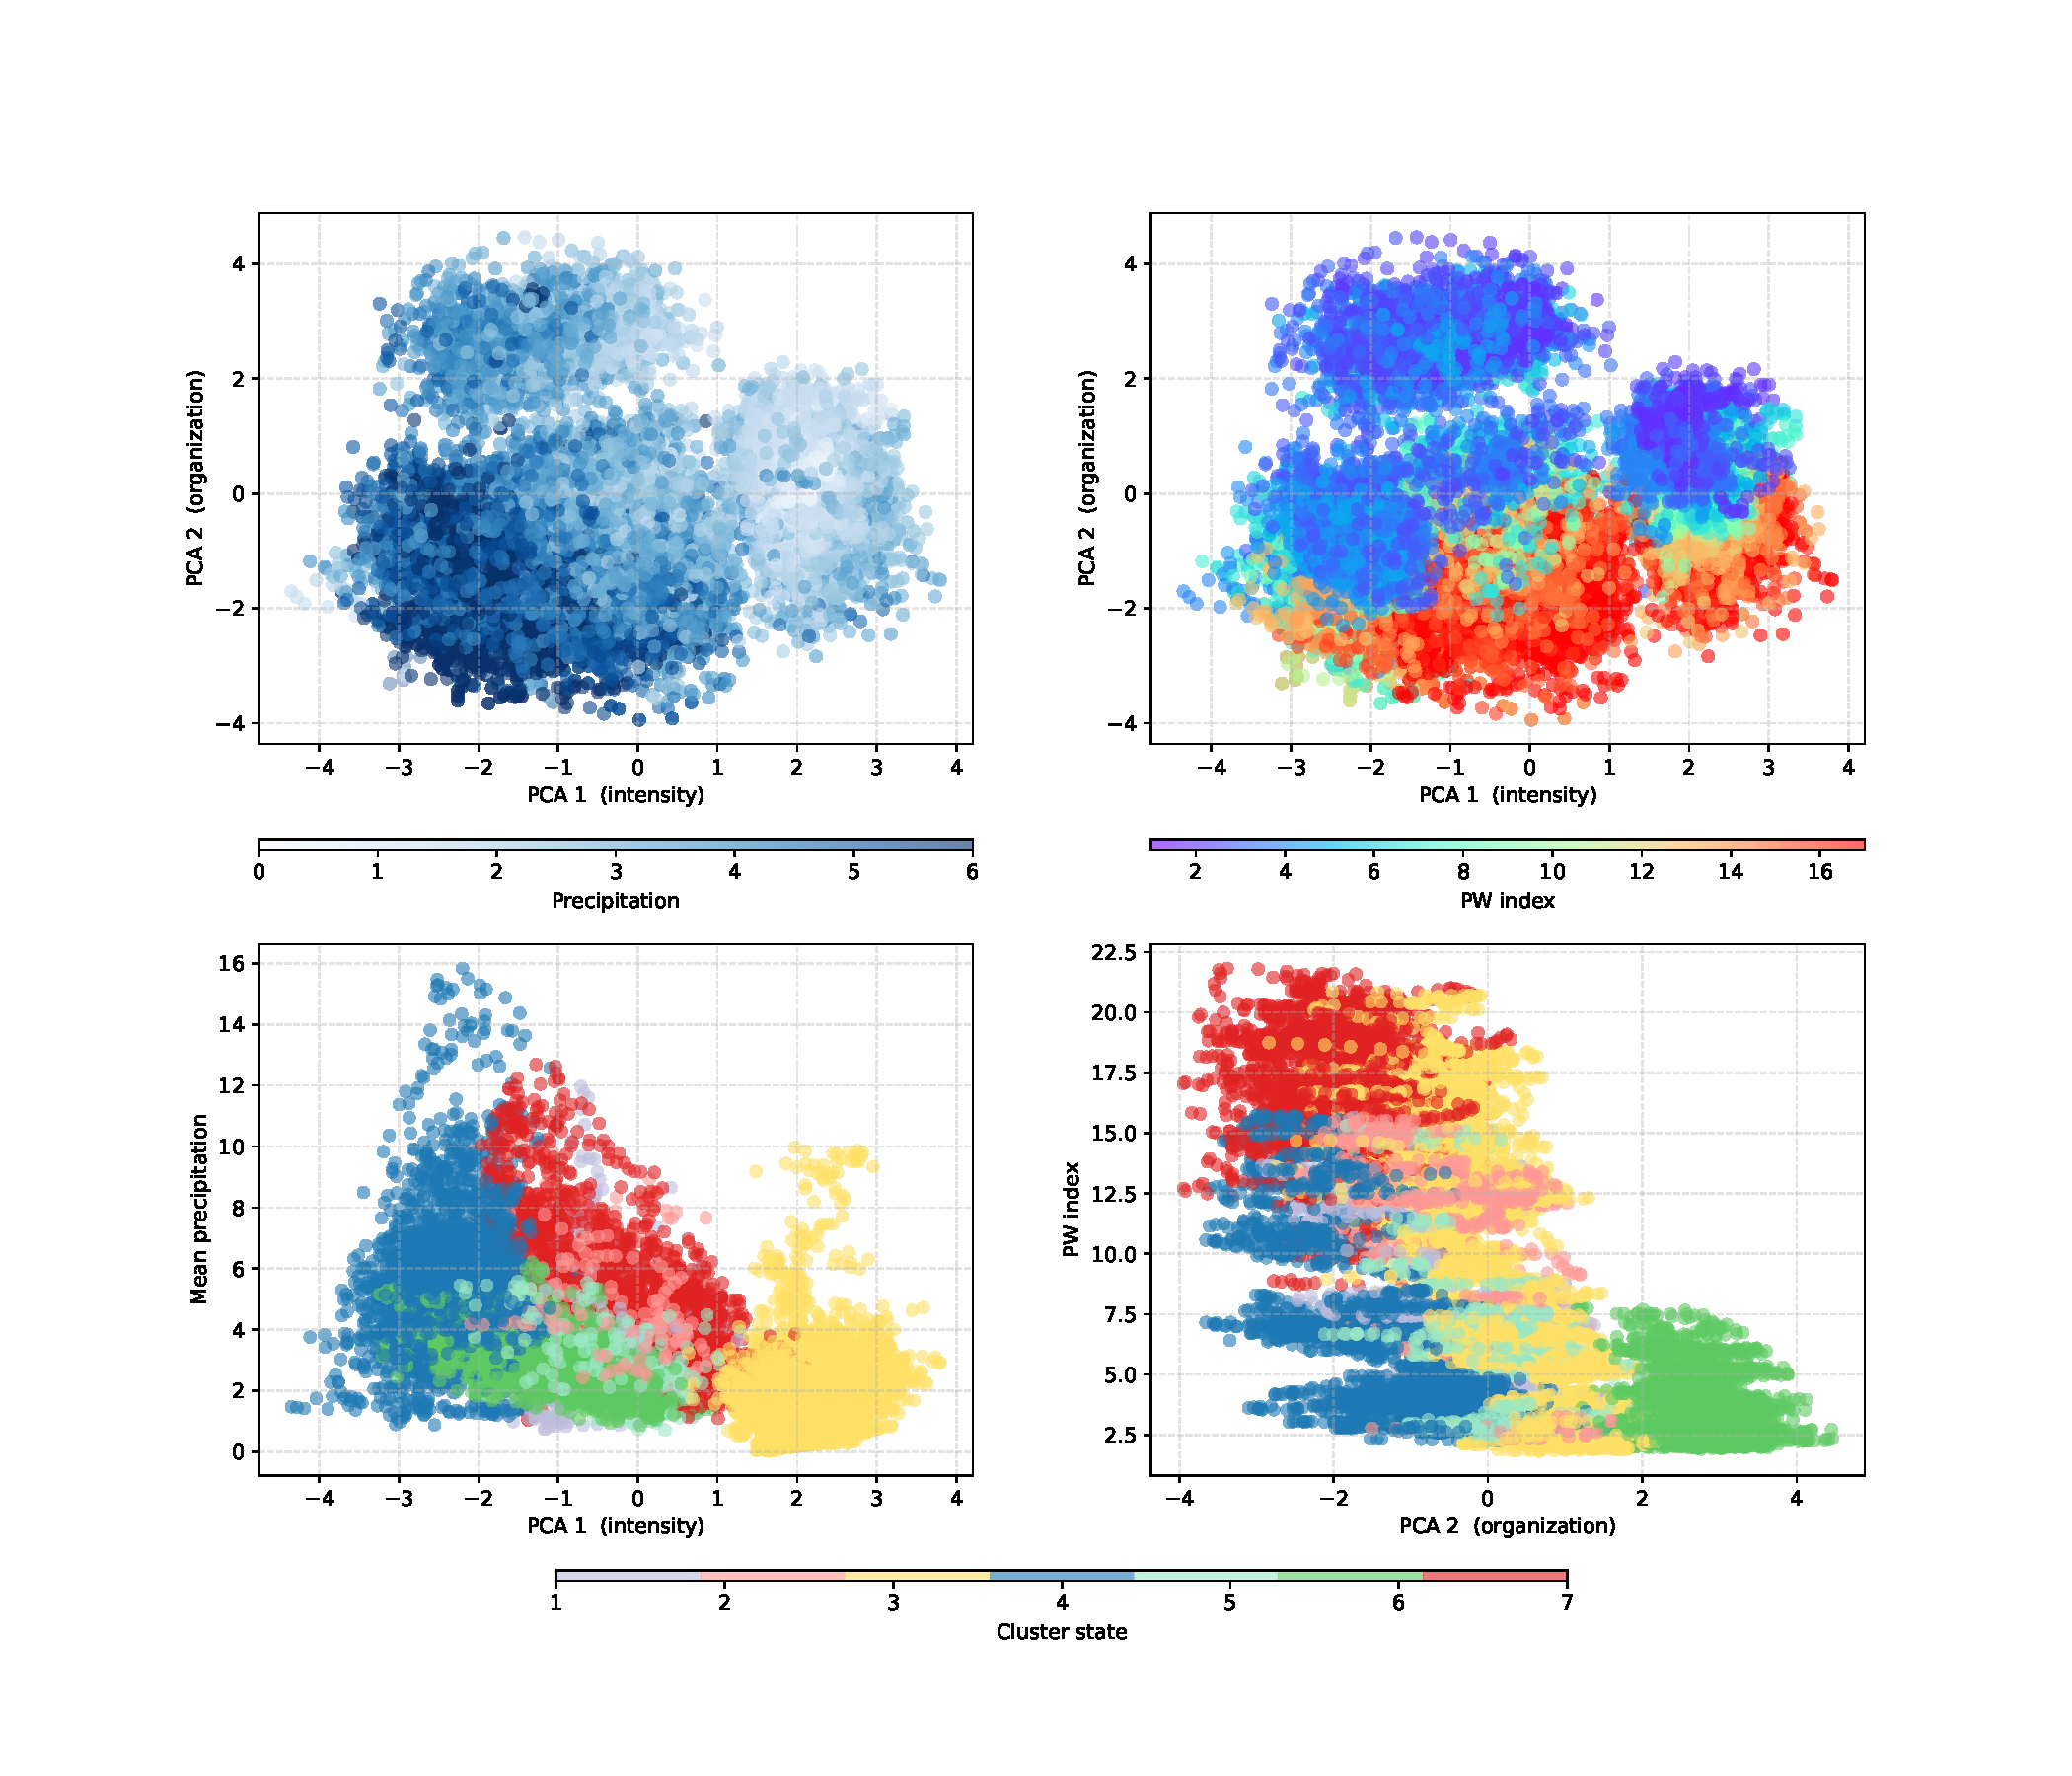
\includegraphics[width=0.95\linewidth]{latent_axis.pdf}
    \caption{\textbf{Physical interpretation of latent variability.} PCA projection colored by (A) mean precipitation and (B) organization index. (C--D) Joint distributions of the first two principal components with the corresponding diagnostics.}
    \label{fig:axis_var}
\end{figure}

\paragraph{Dynamical and thermodynamic signatures of latent states.}

If the latent clusters correspond to physically meaningful convective regimes, they should be associated with systematic differences in vertical mass transport and thermodynamic structure. Representative isentropic mass-flux fields for each cluster are shown in Supplementary Fig.~S3.

Let $M(h,z,t)$ denote the isentropic mass flux at time $t$, height $z$, and moist static energy $h$. For each cluster $c$, we define the cluster-mean vertically integrated positive and negative mass fluxes,
\begin{equation}
M^{\pm}_c(z)
=
\left\langle
\int_h M(h,z,t)\,\mathbf{1}\{\pm M>0\}
\right\rangle_{t\in c},
\end{equation}
and anomalies relative to the simulation-wide mean profiles $\overline{M}^{\pm}(z)$,
\begin{equation}
\Delta^{\pm}_c(z)
=
M^{\pm}_c(z)-\overline{M}^{\pm}(z),
\qquad
\Delta^{\mathrm{net}}_c(z)
=
\Delta^{+}_c(z)-\Delta^{-}_c(z).
\end{equation}

The resulting vertical profiles (Fig.~\ref{fig:vertical_profiles}) reveal clear dynamical distinctions between clusters. States separated primarily along the intensity axis differ mainly in the magnitude of both upward and downward mass flux throughout the troposphere. Cluster~2 exhibits weak updrafts and downdrafts, consistent with shallow or weak convection, whereas Cluster~3 shows enhanced updraft--downdraft coupling characteristic of intense, precipitation-driven convection. Cluster~6 displays the strongest net upward mass transport over much of the troposphere, consistent with sustained deep convection.

\begin{figure}
    \centering
    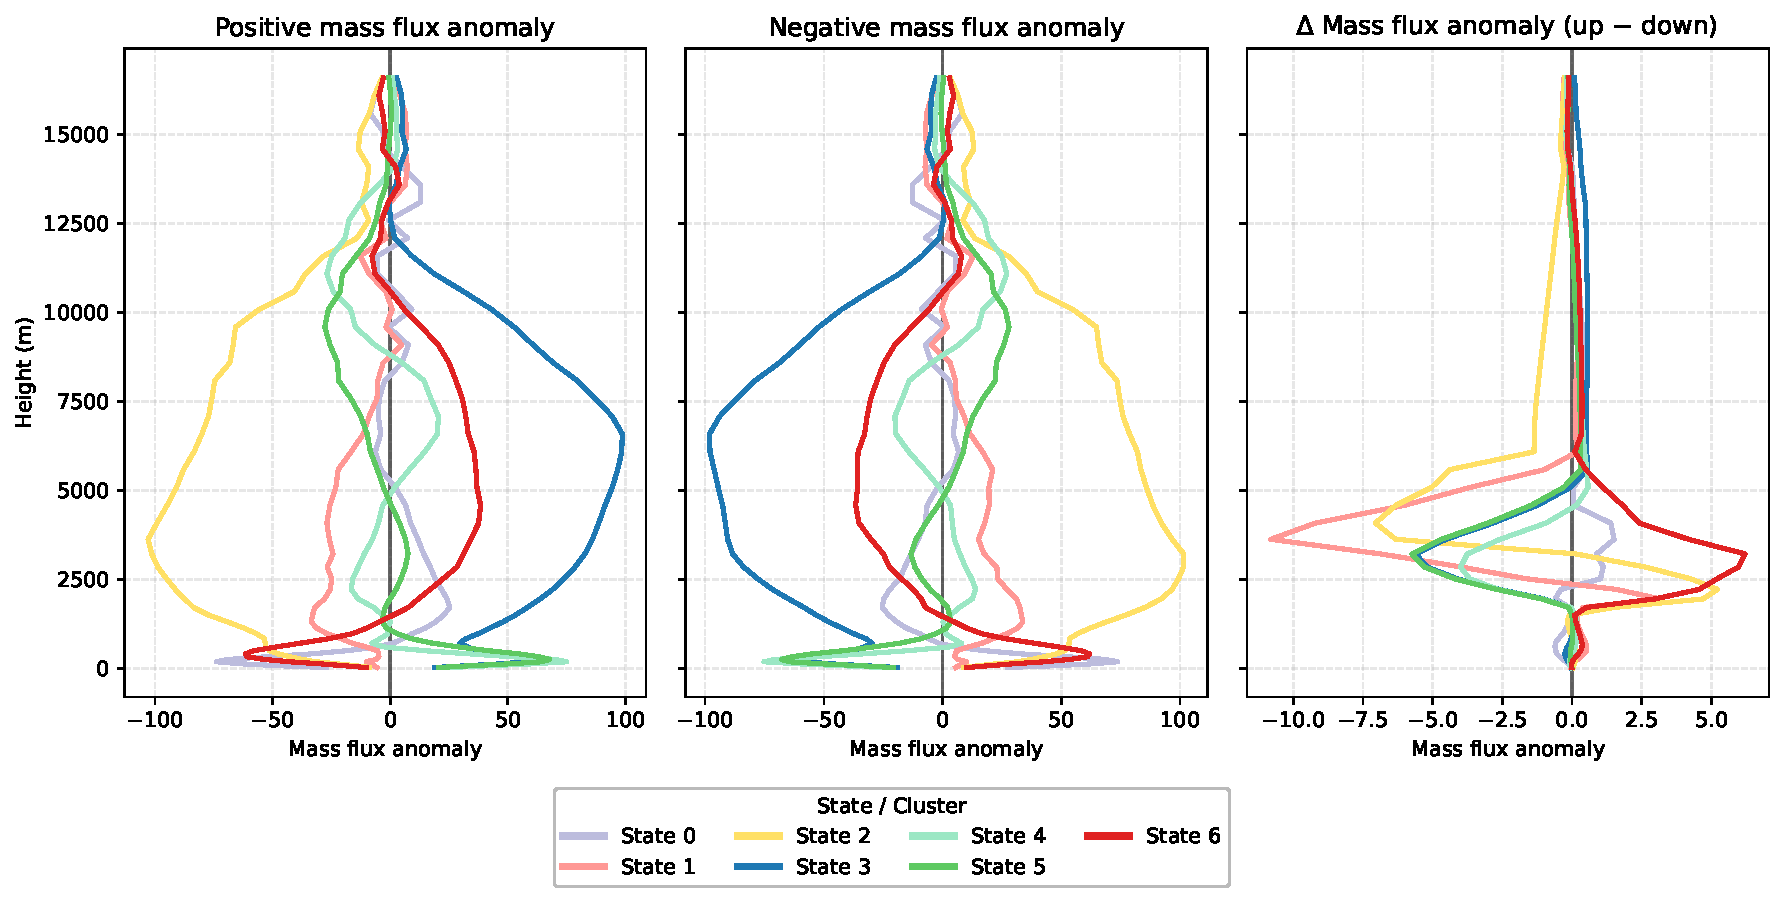
\includegraphics[width=\textwidth]{vertical_profiles.pdf}
    \caption{\textbf{Cluster-averaged vertical mass-flux anomalies.} Positive, negative, and net anomalies relative to the simulation-wide mean.}
    \label{fig:vertical_profiles}
\end{figure}

Thermodynamic differences associated with convective organization are evident in the distribution of mass-flux anomalies across moist static energy (Fig.~\ref{fig:mse_profiles}). Organized states, notably Cluster~6, exhibit enhanced positive mass flux at high moist static energy, indicative of reduced entrainment and enhanced buoyancy within coherent convective structures. Less organized states show anomalies concentrated at lower energy levels, consistent with stronger entrainment and more transient convection.

\begin{figure}
    \centering
    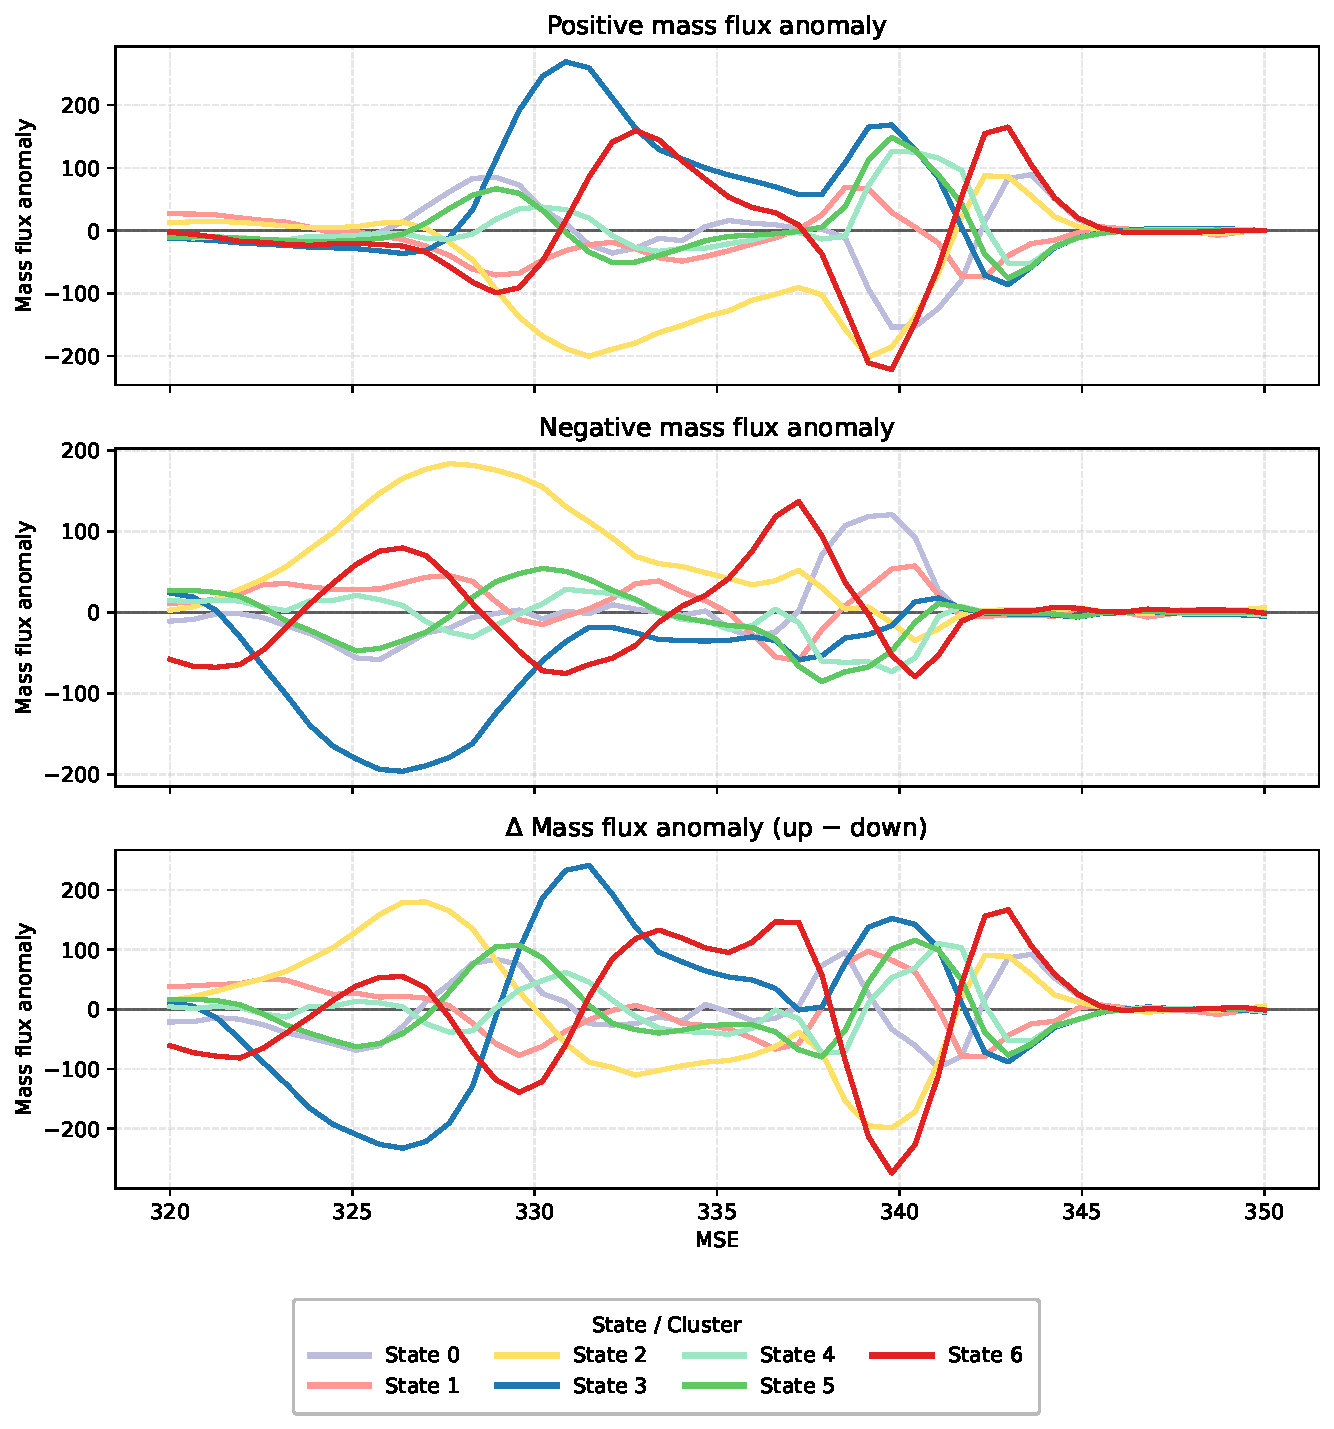
\includegraphics[width=\textwidth]{mse_profiles.pdf}
    \caption{\textbf{Cluster-averaged moist static energy--resolved mass-flux anomalies.}}
    \label{fig:mse_profiles}
\end{figure}

Together, these results show that the VAE latent space organizes convective variability along two emergent and physically interpretable axes—intensity and organization—and that the resulting discrete latent states correspond to dynamically and thermodynamically distinct convective regimes.

\subsection{Markov transition matrix, eigenmodes, and regimes}

The second output of the model is a Markov transition matrix $\mathbf{T}$, whose elements
\begin{equation}
T_{ij} = \mathbb{P}\left( X_{t+\Delta t} = j \mid X_t = i \right)
\end{equation}
denote the probability of transitioning from state $i$ to state $j$. Although the data are sampled at a native temporal resolution of $\Delta t = 2\,\mathrm{min}$, transitions are evaluated at a coarser 10-min interval by considering a 5-step transition matrix. The resulting transition matrix is shown in Fig.~\ref{fig:markov_matrix}.

The matrix $\mathbf{T}$ is strongly diagonally dominated, indicating that the
system tends to persist within a given state over several time steps.
Moreover, the matrix is sparse, with only a limited number of preferred transitions
between states, suggesting constrained pathways in state space.

To further characterize the dynamics, we perform a spectral decomposition of
$\mathbf{T}$.
Because $\mathbf{T}$ is stochastic, it admits a unit eigenvalue $\lambda_1=1$. The corresponding right eigenvector $\boldsymbol{\pi}$ satisfies $\mathbf{T}\boldsymbol{\pi}=\boldsymbol{\pi}$ and defines the stationary distribution of the Markov chain. We obtain
\begin{equation}
\boldsymbol{\pi} =
\begin{bmatrix}
4.7\% & 4.9\% & 36.4\% & 18.0\% & 2.9\% & 20.2\% & 12.8\%
\end{bmatrix}.
\label{eq:canon}
\end{equation}

The stationary distribution is dominated by Cluster~2 ($36.4\%$), followed by Clusters~5 ($20.2\%$),~3 ($18.0\%$), and~6 ($12.8\%$). Clusters~0 ($4.7\%$),~1 ($4.9\%$), and~4 ($2.9\%$ are rarely occupied.

We next examine the subdominant eigenvalues and eigenvectors of
$\mathbf{T}$.
All eigenvalues are real; no complex conjugate pairs are found, despite the
expectation that oscillatory behavior might be present.
This indicates that the dominant dynamics cannot be described as simple linear
oscillations in state space.

The leading nontrivial eigenvalue of the transition matrix is
\begin{equation}
\lambda_2 \approx 0.93,
\end{equation}
indicating a highly persistent dynamical mode. The corresponding eigenvector
\begin{equation}
\mathbf{v}_2 =
\begin{bmatrix}
2.1$\%$ & -12.6$\%$ & 55.5$\%$ & -47.6$\%$ & -2.5$\%$ & -44.7$\%$ & 49.8$\%$
\end{bmatrix}
\end{equation}
describes deviations from the stationary distribution. Positive (negative) components of $\mathbf{v}_2$ indicate enhanced (suppressed) occupancy of the corresponding states relative to $\boldsymbol{\pi}$.

This eigenmode separates the dynamics into two contrasting regimes. In the positive phase of the mode, Clusters~2 and~6 are preferentially occupied, while Clusters~3 and~5 are suppressed. In the negative phase, Clusters~3 and~5 are enhanced at the expense of Cluster~6, with the remaining clusters exhibiting comparatively weak variations (amplitudes $\leq 0.1$). These two regimes are also apparent directly in the structure of the transition matrix $\mathbf{T}$.

Physically, these two regimes correspond to distinct modes of convective evolution.
The first regime represents a directly organized convective system, while the
second regime describes a trajectory that passes through unorganized,
popcorn-like convection before dissipating.
Time series of individual realizations confirm that system trajectories cluster along these two pathways, consistent with the structures inferred from the transition matrix and its leading eigenmodes.

We next assess whether the clustered dynamics are approximately Markovian, and thus whether the transition matrix alone captures the dominant regime evolution. Potential deviations may arise from slow processes, such as moisture memory, not represented in the state partition.


\begin{figure}
    \centering
    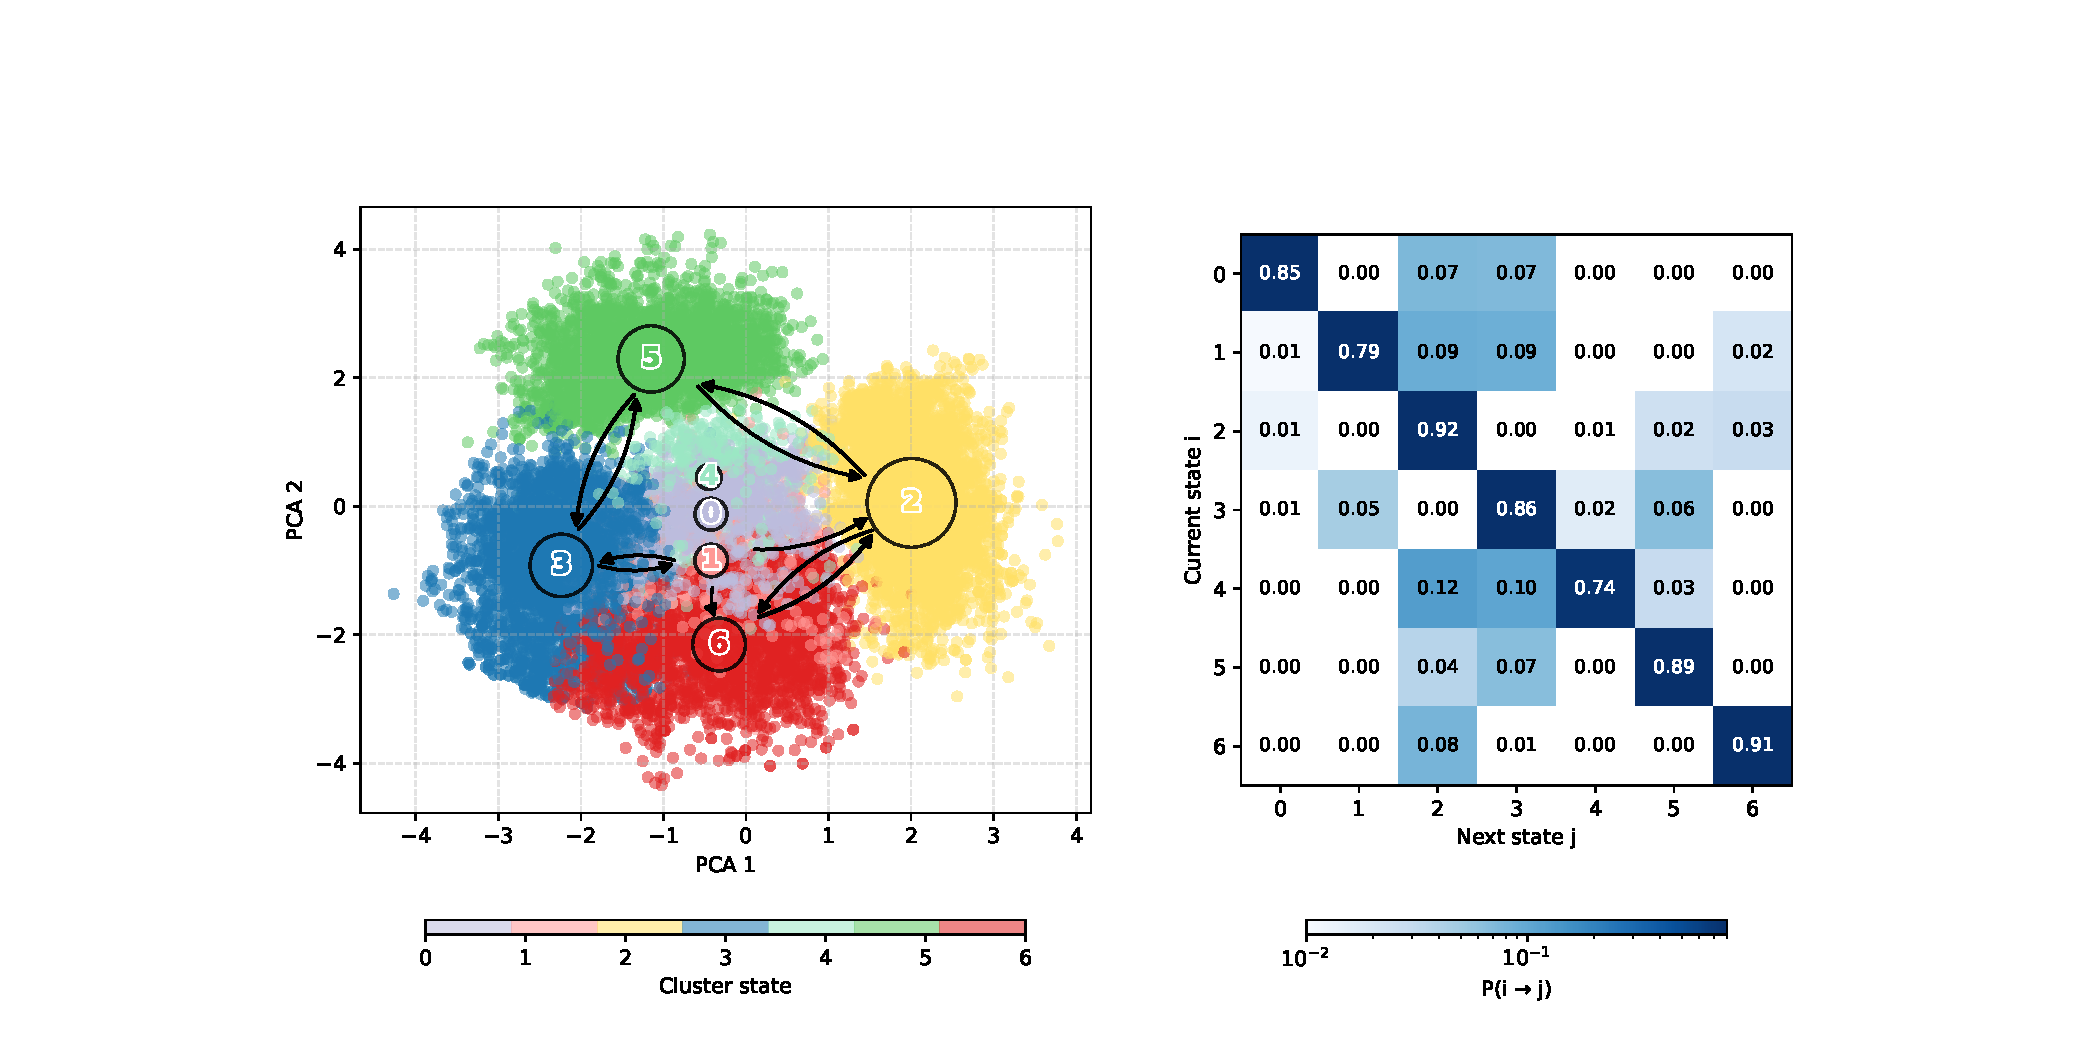
\includegraphics[width=\textwidth]{markov_matrix.pdf}
    \caption{\textbf{Markov state dynamics in latent space.} \textbf{(A)} Latent space visualization with the inferred Markov chain overlaid. The size of each state node is proportional to its asymptotic (stationary) probability, and arrows indicate transition probabilities between states. For clarity, transitions involving States~0 and~4 are omitted, as they play a limited role in the identified convective regimes. \textbf{(B)} Transition matrix describing the dynamics of convection under a given shear. The dominance of the diagonal indicates strong state persistence, with the system remaining in a given state for extended periods. Analysis of the transition structure reveals preferred pathways, including oscillations among States~2--5--3 associated with weakly organized convection, and transitions between States~2 and~6 associated with strongly organized convection. The matrix further indicates that transitions from weakly to strongly organized convection preferentially occur via the intermediate State~1.}
    \label{fig:markov_matrix}
\end{figure}

\subsection{Markovianity assessment and internal feedbacks}

We finally assess the extent to which the inferred state dynamics can be approximated as Markovian, and thus whether the chosen state partitioning provides a self-contained description of the system’s temporal evolution.
Under the Markov hypothesis, the state at time $t$ contains all the information required to predict the state at time $t+1$, implying that memory of earlier states does not contribute to the near-future dynamics. Deviations from this assumption would indicate the presence of unresolved internal feedbacks or slow processes—such as moisture memory or large-scale environmental modulation—that are not explicitly captured by the clustering.

A standard approach to test Markovianity is through the analysis of temporal autocorrelations. For a Markov process, correlations between the present state and states at increasing time lags are expected to decay exponentially, reflecting the progressive loss of information about past configurations.

\paragraph{State indicator autocorrelation.}
We introduce the indicator function associated with state $i$,
\begin{equation}
I_i(t) = \mathbf{1}[X_t = i],
\end{equation}
and define the normalized autocorrelation function
\begin{equation}
C_i(\tau) =
\frac{
\mathbb{E}\left[(I_i(t)-\pi_i)(I_i(t+\tau)-\pi_i)\right]
}{
\mathbb{E}\left[(I_i(t)-\pi_i)^2\right]
},
\end{equation}
where $\mathbb{E}[\cdot]$ is the expectation, $\pi_i$ is the stationary probability of state $i$ (see \ref{eq:canon}), noting that $\mathbb{E}[I_i(t)] = \pi_i$ under stationarity.

This quantity measures how strongly the occupancy of state $i$ at time $t$ influences the probability of occupying the same state at a later time $t+\tau$.

\paragraph{Expected behavior for a Markov chain.}
Assume that ${X_t}$ is a discrete-time Markov chain with transition matrix $\mathbf{T}$ and stationary distribution $\boldsymbol{\pi}$. Under stationarity,
\begin{equation}
\mathbb{P}(X_t=i, X_{t+\tau}=i)
= \pi_i T^\tau_{ii},
\end{equation}
and $\mathbb{E}[I_i(t)] = \mathbb{E}[I_i(t+\tau)] = \pi_i$. It follows that
\begin{equation}
C_i(\tau)
= \frac{T^\tau_{ii} - \pi_i}{1-\pi_i}.
\end{equation}

To analyze the temporal structure of $C_i(\tau)$, we use the spectral decomposition of the transition matrix. Denoting the eigenvalues of $\mathbf{T}$ by $(1,\lambda_2,\dots,\lambda_K)$, the leading eigenvalue $\lambda_1=1$ corresponds to the stationary distribution, while all other eigenvalues satisfy $|\lambda_\alpha|<1$ for $\alpha\ge 2$. Raising $\mathbf{T}$ to the power $\tau$ yields
\begin{equation}
T^\tau
= \mathbf{1}\boldsymbol{\pi}^\top
+ \sum_{\alpha=2}^K \lambda_\alpha^\tau  v_\alpha w_\alpha^\top,
\end{equation}
where $\mathbf{v}_\alpha$ and $\mathbf{w}_\alpha$ denote the right and left eigenvectors of $\mathbf{T}$ associated with the eigenvalue $\lambda_\alpha$, respectively, normalized such that $\mathbf{w}_\alpha^\top \mathbf{v}_\beta = \delta_{\alpha\beta}$. In particular $w_1=\pi$ and $v_1=(1, 1, .., 1)$.

Substituting into the expression for $C_i(\tau)$, the stationary contribution cancels exactly, leading to
\begin{equation}
C_i(\tau)
= \sum_{\alpha=2}^K A_\alpha^{(i)} \lambda_\alpha^\tau ,
\label{eq:autocor} 
\end{equation}
where $A_\alpha^{(i)}
=
\left(\mathbf{e}_i^\top \mathbf{v}_\alpha\right)
\left(\mathbf{w}_\alpha^\top \mathbf{e}_i\right)
/
(1 - \pi_i)
$

Thus, for a Markovian system, the state autocorrelation function is a superposition of exponentially decaying modes. At sufficiently large time lags, the decay is dominated by the second-largest eigenvalue,
\begin{equation}
C_i(\tau) \sim \lambda_2^\tau
= \exp\left(-\tau / \tau_{\mathrm{corr}}\right),
\end{equation}
with correlation time $\tau_{\mathrm{corr}} = -1/\ln|\lambda_2|$. The step by step proof can be found in the supplementary.

Exponential decay of state autocorrelations therefore provides a direct and quantitative test of the Markov assumption. Systematic departures from this behavior indicate residual memory effects and suggest that the chosen partition does not fully isolate the relevant dynamical degrees of freedom.

\paragraph{Diagnosis of memory effects.}
Departures from exponential decay indicate either genuinely non-Markovian dynamics or an incomplete state representation in which slow variables have been omitted.
We therefore compute the indicator autocorrelation $C_i(\tau)$ for each state and compare it to the theoretical Markovian prediction derived from the estimated transition matrix.

Figure~\ref{fig:autocorrelation} shows the empirical autocorrelations (solid lines) together with the Markovian expectation from \ref{eq:autocor} (dashed lines). 
Most states exhibit a rapid decay consistent with Markovian dynamics. 
However, states corresponding to shallow convection (state~0), popcorn convection (state~5), and organized deep convection (state~6) display significantly slower decay, indicating the presence of memory effects.

\paragraph{Role of internal feedbacks.}
We interpret the observed deviations from Markovian behavior as signatures of internal feedback processes that are not resolved by the discrete state partition. In particular, for state~6, we hypothesize that variability in cold pool activity introduces an additional, slowly evolving internal degree of freedom.

To test this hypothesis, we refine the analysis by conditioning state~6 on a cold pool activity index. This index is constructed by tracking cold pools in time using sea surface temperature anomalies and defining the cold pool activity at each time step as the mean detected cold pool size weighted by its intensity (see Supplementary Information for details).

We then compute state autocorrelations separately for occurrences of state~6 associated with strong and weak cold pool activity. When conditioned in this manner, the autocorrelations decay rapidly and closely follow the Markovian prediction.

This result indicates that the apparent non-Markovian behavior of state~6 originates from unresolved internal feedback variability rather than a breakdown of the Markov framework itself. Incorporating cold pool activity into the state description therefore provides a physically motivated pathway toward a more Markovian representation of the convective dynamics.

\begin{figure}
    \centering
    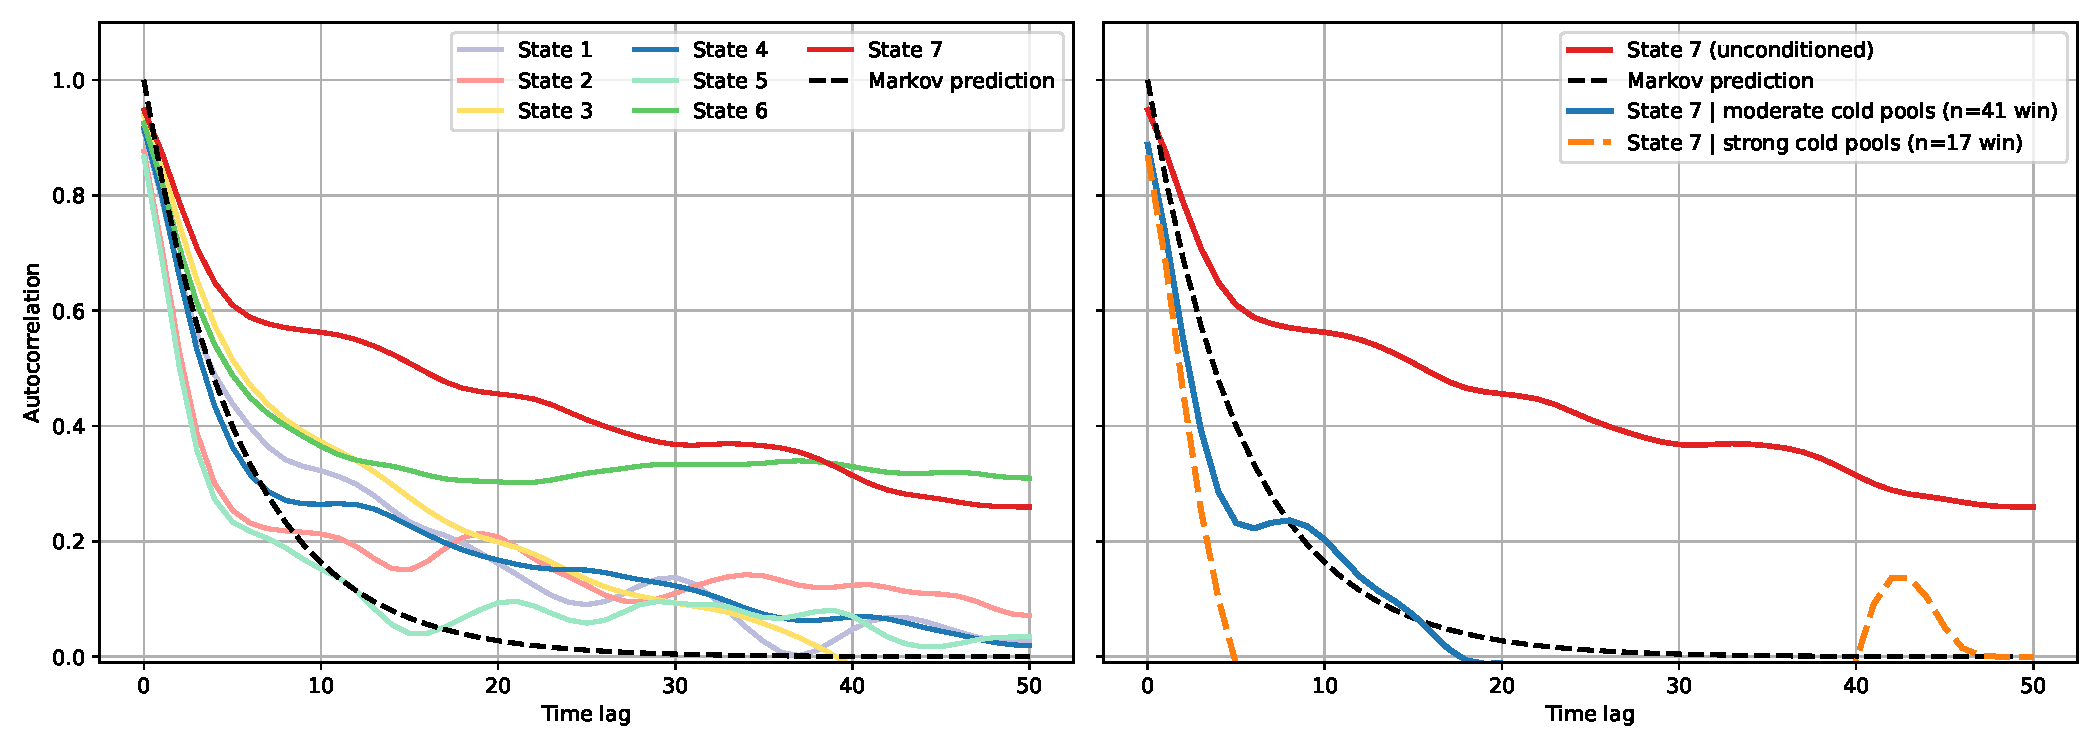
\includegraphics[width=\textwidth]{markovianity_and_coldpools.pdf}
    \caption{(A) State autocorrelation functions (colors) compared with the Markovian prediction from the inferred transition matrix (dashed). Most states exhibit rapid, near-exponential decay, while States~0,~5, and~6 show slower decay and systematic deviations, indicating departures from Markovianity.
(B) Autocorrelation of State~6. Conditioning on cold pool activity (below/above median) yields decay rates consistent with the Markovian prediction, indicating that the apparent non-Markovian behavior arises from unresolved internal variability.
}
    \label{fig:autocorrelation}
\end{figure}


\section{Conclusion}
This work introduces a stochastic, data-driven framework to characterize convective organization through the vertical structure of the isentropic mass flux. Using idealized high-resolution simulations under fixed large-scale forcing and prescribed vertical wind shear, we show that convective mass-flux variability evolves on a low-dimensional manifold and can be compactly represented within an eight-dimensional latent space. This reduced representation provides a dynamically meaningful description of convective variability while retaining the essential structure of vertical transport.\\


Within this latent space, convective dynamics organize into a small number of states associated with distinct phases of the convective life cycle: initiation or rest, intermittent convection, organized convection, and dissipation. The leading directions of variability capture both the temporal evolution of convection and its degree of organization, while intermediate regions correspond to transition pathways between these states. This new representation offers a process-oriented view of convection that moves beyond horizontal cloud-type classifications.\\


We further demonstrate that convective evolution in this reduced space can be described as a stochastic process governed by a Markov transition matrix. This probabilistic description reveals preferred regimes, canonical distributions, and characteristic time scales, and distinguishes organized from unorganized modes of convection. Autocorrelation analysis shows that organized convective states exhibit memory effects, indicating departures from strict Markovian behavior. Conditioning the state space on an external cold-pool index improves Markovianity, highlighting the role of internal feedbacks in shaping convective pathways and emphasizing the importance of incorporating such processes into stochastic representations of convection.


\section{Discussion}
\paragraph{Internal feedbacks and state construction.}

The results highlight the central role of internal convective feedbacks in governing state-to-state evolution. Processes such as cold-pool dynamics, entrainment, and mesoscale circulations introduce memory and nonlocal interactions that are not fully captured by purely Markovian state descriptions. Although isentropic coordinates are expected to capture cold-pool anomalies, their signature is not clearly isolated here, potentially reflecting limited signal strength or sensitivity to the binning of moist static energy. Overall, the results suggest that while external forcing constrains the accessible state space, internal feedbacks regulate the trajectories within it, underscoring the importance of embedding such feedbacks directly in stochastic state definitions.\\


\paragraph{Influence of external forcing on latent structure and transitions.}
An important open question concerns how external forcing shapes the geometry of the latent space and the associated transition dynamics. Changes in environmental parameters such as vertical wind shear are expected to modify both the accessible convective states and the probabilities of transitions between them. Comparing latent spaces and transition matrices across different forcing regimes offers a systematic framework for assessing forcing dependence and for identifying common structures that persist across environments. 


\paragraph{The dynamical nature of convective organization.}
A key strength of the proposed framework is that convective organization is characterized dynamically, as trajectories through a reduced state space, rather than solely through static or time-averaged diagnostics. In this view, organized convection is defined not only by the states it occupies, but by the sequences of transitions through which it emerges, persists, and decays. This trajectory-based perspective enables direct comparison of convective systems with similar bulk properties but distinct temporal evolutions, and provides a dynamical foundation for studying convective organization as an evolving process rather than a static outcome. Taken together, these results suggest that diversity emerges from the range of trajectories promoted by large-scale forcing, rather than from the presence of distinct states alone.

\section{Data and Code Availability}

The simulations analyzed in this study consist of idealized squall-line simulations performed with the System for Atmospheric Modeling (SAM). The dataset spans 27 days of simulation at 2-minute temporal resolution and includes one-dimensional, two-dimensional, and three-dimensional model outputs. The data are available via Globus (link to be provided).

All code used in this study is openly available at: \url{https://github.com/sososquirrel/troposwhere}. The repository includes the implementation of the model as well as the scripts required to reproduce all figures presented in the paper.

\section{Acknowledgments}

The authors thank Sara Shamekh for helpful feedback on this work. We are grateful to Juan Nathanael and Carla Roesch for discussions on Koopman operators, and to Fabrizio Falasca and Matthieu Blanke for recommendations on the dynamical systems literature. We also thank Zhe Feng, Xingchao Chen, Ruby Leung, and the WACCEM project team for valuable discussions throughout the course of this study.

Portions of the manuscript were rephrased with the assistance of ChatGPT (OpenAI) for language editing, and Claude (Anthropic) assisted with aspects of code development and cleaning. These tools were used solely to improve clarity and software organization; all scientific ideas, analysis, and conclusions were developed by the authors.


This research was supported by the Office of Science of the U.S. Department of Energy (DOE), Biological and Environmental Research (BER), as part of the Regional and Global Modeling and Analysis program area under the Water Cycle and Climate Extremes Modeling (WACCEM) project.

\section{Author Contributions}

S.A. designed the research, performed the simulations, developed the methods and code, and wrote the manuscript. O.P. contributed to the methodological development, contributed to the code, and participated in the analysis and discussions. P.G. contributed to the interpretation of the results and to writing the manuscript.


\printbibliography
\end{document}



\begin{comment}
    \section{Introduction}

Deep convection plays a central role in the transport of mass, energy, and moisture in Earth’s atmosphere, shaping large-scale circulations and extreme weather [add biblio Roca, Feng, Schumacher, Muller]. Yet even under fixed large-scale forcing, convective systems display striking variability: identical environmental conditions can give rise to cloud systems with widely different lifetimes, spatial extents, and degrees of organization [add Houze, Bony, Roca, Leung, Abramian]. This intrinsic variability challenges deterministic descriptions of convection and raises a fundamental question: what diversity of convective systems can arise under a given large-scale forcing?\\

A common strategy for representing this variability is through stochastic parameterizations, in which convective activity is modeled probabilistically rather than deterministically (e.g., Khouider; Majda; Gentine). In these approaches, convective column state is evolving as a Markov chain, with transitions between a small number of idealized convective states and conditioned on large-scale environmental variables. This framework successfully reproduces realistic variability in convective occurrence across space and time. However, because the state space is primarily defined by horizontal location, such models provide limited constraints on the associated vertical redistribution of mass and energy, which governs extreme precipitation (e.g.,Singh, Muller, Bolot).\\

This limitation reflects another aspect in convective dynamics: horizontal organization does not uniquely determine vertical transport. Under comparable large-scale forcing, convective systems can exhibit distinct horizontal structures while producing similar vertical mass-flux profiles, and conversely, geometrically similar systems may differ substantially in their vertical transport (e.g., Greg Elsaesser; Leung; Xingchao). Geometric descriptors such as cloud type or spatial extent are therefore insufficient to characterize the dynamical impact of convection. \\

In this work, we are interested in representing convection defined in terms of its vertical structure. A full-resolution three-dimensional description of convective mass flux leads to an excessively large and noisy state space, obscuring emergence behavior. We look for reducing horizontal spatial resolution to emphasize vertically structured convective configurations within the domain.\\

To do so, we coarse-grain convective mass flux by thermodynamic state using an isentropic analysis (e.g., Pauluis; Mrowiec; Xingchao). Isentropic coordinates provide a thermodynamically consistent framework linking vertical motion to energetic redistribution, yielding a compact, low-dimensional representation while filtering reversible oscillatory motions such as gravity waves. In this isentropic–altitude framework, convection organizes as coherent patterns in mass-flux space rather than as independent evolution at isolated energy levels. This perspective raises two central questions: what is the effective dimensionality of this space, and which vertically structured mass-flux states and transition pathways are accessible under a given large-scale forcing?\\

Representation learning have recently show its power in mapping the high-dimensional space of isentropic mass-flux fields onto a low-dimensional latent space that preserves the dominant structures of convective transport [paper VAE? representation learning]. This approach provides a natural basis for identifying convective states, quantifying transitions among them, and diagnosing the role of stochasticity and internal feedbacks in shaping convective evolution. In this reduced representation, convective evolution appears as trajectories between distinct regions corresponding to dynamically meaningful convective states. \\

In summary, the objective of this study is to characterize the intrinsic variability of deep convection under fixed large-scale forcing through its vertical transport of mass and energy. By representing convection in a reduced space defined by vertically structured mass flux, we seek to identify the dominant modes of convective organization and the pathways through which systems evolve between them. More precisely, we address three questions:

(i) What are the dominant convective mass-flux states accessible under a given large-scale forcing, here characterized by vertical wind shear?
(ii) Can transitions between these states be modeled as a Markov chain, and do transition pathways differ between weak and strongly organized convection?
(iii) To what extent can convective variability be described by memoryless transitions, and how do internal feedbacks, such as cold-pool dynamics, introduce effective memory?\\
\end{comment}